

\chapter{社会思想の輸入}



\section{『学問のすすめ』(1872-1876)}





「天は人の上に人を造らず人の下に人を造らず」と言えり。されば天より人を生ずるには、万人は万人みな同じ位にして、生まれながら\ruby{貴賤}{きせん}上下の差別なく、万物の霊たる身と心との働きをもって天地の間にあるよろずの物を\ruby{資}{と}り、もって衣食住の用を達し、自由自在、互いに人の妨げをなさずしておのおの安楽にこの世を渡らしめ給うの趣意なり。されども今、広くこの人間世界を見渡すに、かしこき人あり、おろかなる人あり、貧しきもあり、富めるもあり、貴人もあり、下人もありて、その有様雲と\ruby{泥}{どろ}との相違あるに似たるはなんぞや。その次第はなはだ明らかなり。『\ruby{実語教}{じつごきょう}』に、「人学ばざれば智なし、智なき者は愚人なり」とあり。されば賢人と愚人との別は学ぶと学ばざるとによりてできるものなり。また世の中にむずかしき仕事もあり、やすき仕事もあり。そのむずかしき仕事をする者を身分重き人と名づけ、やすき仕事をする者を身分軽き人という。すべて心を用い、心配する仕事はむずかしくして、手足を用うる\ruby{力役}{りきえき}はやすし。ゆえに医者、学者、政府の役人、または大なる商売をする町人、あまたの奉公人を召し使う大百姓などは、身分重くして貴き者と言うべし。

 \begin{figure}[htbp]
   \centering
 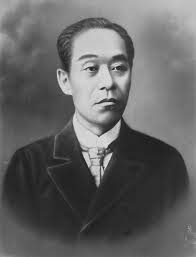
\includegraphics[width=50mm]{images/fukuzawa.jpg}  
   \caption{福沢諭吉}
 \end{figure}


身分重くして貴ければおのずからその家も富んで、\ruby{下々}{しもじも}の者より見れば及ぶべからざるようなれども、その\ruby{本}{もと}を尋ぬればただその人に学問の力あるとなきとによりてその相違もできたるのみにて、天より定めたる約束にあらず。\ruby{諺}{ことわざ}にいわく、「天は富貴を人に与えずして、これをその人の働きに与うるものなり」と。されば前にも言えるとおり、人は生まれながらにして貴賤・貧富の別なし。ただ学問を勤めて物事をよく知る者は貴人となり富人となり、無学なる者は貧人となり\ruby{下人}{げにん}となるなり。

学問とは、ただむずかしき字を知り、\ruby{解}{げ}し難き古文を読み、和歌を楽しみ、詩を作るなど、世上に実のなき文学を言うにあらず。これらの文学もおのずから人の心を\ruby{悦}{よろこ}ばしめずいぶん調法なるものなれども、古来、世間の儒者・和学者などの申すよう、さまであがめ\ruby{貴}{とうと}むべきものにあらず。古来、漢学者に世帯持ちの上手なる者も少なく、和歌をよくして商売に巧者なる町人もまれなり。これがため心ある町人・百姓は、その子の学問に出精するを見て、やがて身代を持ち崩すならんとて親心に心配する者あり。無理ならぬことなり。\ruby{畢竟}{ひっきょう}その学問の実に遠くして日用の間に合わぬ証拠なり。

されば今、かかる実なき学問はまず次にし、もっぱら勤むべきは人間普通日用に近き実学なり。\ruby{譬}{たと}えば、いろは四十七文字を習い、手紙の\ruby{文言}{もんごん}、帳合いの仕方、\ruby{算盤}{そろばん}の稽古、\ruby{天秤}{てんびん}の取扱い等を心得、なおまた進んで学ぶべき箇条ははなはだ多し。地理学とは日本国中はもちろん世界万国の\ruby{風土}{ふうど}道案内なり。究理学とは天地万物の性質を見て、その働きを知る学問なり。歴史とは年代記のくわしきものにて万国古今の有様を詮索する書物なり。経済学とは一身一家の世帯より天下の世帯を説きたるものなり。修身学とは身の行ないを修め、人に交わり、この世を渡るべき天然の道理を述べたるものなり。

これらの学問をするに、いずれも西洋の翻訳書を取り調べ、たいていのことは日本の仮名にて用を便じ、あるいは年少にして文才ある者へは横文字をも読ませ、一科一学も実事を押え、その事につきその物に従い、近く物事の道理を求めて今日の用を達すべきなり。右は人間普通の実学にて、人たる者は貴賤上下の区別なく、みなことごとくたしなむべき心得なれば、この心得ありて後に、士農工商おのおのその分を尽くし、銘々の家業を営み、身も独立し、家も独立し、天下国家も独立すべきなり。

学問をするには分限を知ること肝要なり。人の天然生まれつきは、繋つながれず縛られず、\ruby{一人前}{いちにんまえ}の男は男、一人前の女は女にて、自由自在なる者なれども、ただ自由自在とのみ唱えて\ruby{分限}{ぶんげん}を知らざればわがまま放蕩に陥ること多し。すなわちその分限とは、天の道理に基づき人の情に従い、他人の妨げをなさずしてわが一身の自由を達することなり。自由とわがままとの\ruby{界}{さかい}は、他人の妨げをなすとなさざるとの間にあり。\ruby{譬}{たと}えば自分の金銀を費やしてなすことなれば、たとい酒色に\ruby{耽}{ふけ}り放蕩を尽くすも自由自在なるべきに似たれども、けっして然しからず、一人の放蕩は諸人の手本となり、ついに世間の風俗を乱りて人の教えに妨げをなすがゆえに、その費やすところの金銀はその人のものたりとも、その罪許すべからず。

また自由独立のことは人の一身にあるのみならず、一国の上にもあることなり。わが日本はアジヤ州の東に離れたる一個の島国にて、古来外国と交わりを結ばず、ひとり自国の産物のみを衣食して不足と思いしこともなかりしが、嘉永年中アメリカ人渡来せしより外国\ruby{交易}{こうえき}のこと始まり、今日の有様に及びしことにて、開港の後もいろいろと議論多く、鎖国\ruby{攘夷}{じょうい}などとやかましく言いし者もありしかども、その見るところはなはだ狭く、\ruby{諺}{ことわざ}に言う「井の底の蛙かわず」にて、その議論とるに足らず。日本とても西洋諸国とても同じ天地の間にありて、同じ日輪に照らされ、同じ月を眺め、海をともにし、空気をともにし、情合い相同じき人民なれば、ここに余るものは彼に渡し、彼に余るものは我に取り、互いに相教え互いに相学び、恥ずることもなく誇ることもなく、互いに便利を達し互いにその幸いを祈り、天理人道に従いて互いの交わりを結び、理のためにはアフリカの\ruby{黒奴}{こくど}にも恐れ入り、道のためにはイギリス・アメリカの軍艦をも恐れず、国の恥辱とありては日本国中の人民一人も残らず命を\ruby{棄}{す}てて国の威光を落とさざるこそ、一国の自由独立と申すべきなり。〔……〕


\if0
しかるを支那人などのごとく、わが国よりほかに国なきごとく、外国の人を見ればひとくちに夷狄いてき夷狄と唱え、四足にてあるく畜類のようにこれを賤いやしめこれを嫌きらい、自国の力をも計らずしてみだりに外国人を追い払わんとし、かえってその夷狄に窘くるしめらるるなどの始末は、実に国の分限を知らず、一人の身の上にて言えば天然の自由を達せずしてわがまま放蕩に陥る者と言うべし。王制一度ひとたび新たなりしより以来、わが日本の政風大いに改まり、外は万国の公法をもって外国に交わり、内は人民に自由独立の趣旨を示し、すでに平民へ苗字みょうじ・乗馬を許せしがごときは開闢かいびゃく以来の一美事びじ、士農工商四民の位を一様にするの基もといここに定まりたりと言うべきなり。

されば今より後は日本国中の人民に、生まれながらその身につきたる位などと申すはまずなき姿にて、ただその人の才徳とその居処きょしょとによりて位もあるものなり。たとえば政府の官吏を粗略にせざるは当然のことなれども、こはその人の身の貴きにあらず、その人の才徳をもってその役儀を勤め、国民のために貴き国法を取り扱うがゆえにこれを貴ぶのみ。人の貴きにあらず、国法の貴きなり。旧幕府の時代、東海道にお茶壺の通行せしは、みな人の知るところなり。そのほか御用の鷹たかは人よりも貴く、御用の馬には往来の旅人も路を避くる等、すべて御用の二字を付くれば、石にても瓦かわらにても恐ろしく貴きもののように見え、世の中の人も数千百年の古いにしえよりこれを嫌いながらまた自然にその仕来しきたりに慣れ、上下互いに見苦しき風俗を成せしことなれども、畢竟これらはみな法の貴きにもあらず、品物の貴きにもあらず、ただいたずらに政府の威光を張り人を畏おどして人の自由を妨げんとする卑怯なる仕方にて、実なき虚威というものなり。今日に至りてはもはや全日本国内にかかる浅ましき制度、風俗は絶えてなきはずなれば、人々安心いたし、かりそめにも政府に対して不平をいだくことあらば、これを包みかくして暗に上かみを怨うらむることなく、その路を求め、その筋により静かにこれを訴えて遠慮なく議論すべし。天理人情にさえ叶うことならば、一命をも抛なげうちて争うべきなり。これすなわち一国人民たる者の分限と申すものなり。

前条に言えるとおり、人の一身も一国も、天の道理に基づきて不覊ふき自由なるものなれば、もしこの一国の自由を妨げんとする者あらば世界万国を敵とするも恐るるに足らず、この一身の自由を妨げんとする者あらば政府の官吏も憚はばかるに足らず。ましてこのごろは四民同等の基本も立ちしことなれば、いずれも安心いたし、ただ天理に従いて存分に事をなすべしとは申しながら、およそ人たる者はそれぞれの身分あれば、またその身分に従い相応の才徳なかるべからず。身に才徳を備えんとするには物事の理を知らざるべからず。物事の理を知らんとするには字を学ばざるべからず。これすなわち学問の急務なるわけなり。

昨今の有様を見るに、農工商の三民はその身分以前に百倍し、やがて士族と肩を並ぶるの勢いに至り、今日にても三民のうちに人物あれば政府の上に採用せらるべき道すでに開けたることなれば、よくその身分を顧み、わが身分を重きものと思い、卑劣の所行あるべからず。およそ世の中に無知文盲の民ほど憐あわれむべくまた悪にくむべきものはあらず。智恵なきの極きわみは恥を知らざるに至り、己おのが無智をもって貧窮に陥り飢寒に迫るときは、己が身を罪せずしてみだりに傍かたわらの富める人を怨み、はなはだしきは徒党を結び強訴ごうそ・一揆いっきなどとて乱暴に及ぶことあり。恥を知らざるとや言わん、法を恐れずとや言わん。天下の法度ほうどを頼みてその身の安全を保ち、その家の渡世をいたしながら、その頼むところのみを頼みて、己が私欲のためにはまたこれを破る、前後不都合の次第ならずや。あるいはたまたま身本みもと慥たしかにして相応の身代ある者も、金銭を貯たくわうることを知りて子孫を教うることを知らず。教えざる子孫なればその愚なるもまた怪しむに足らず。ついには遊惰放蕩に流れ、先祖の家督をも一朝の煙となす者少なからず。

かかる愚民を支配するにはとても道理をもって諭さとすべき方便なければ、ただ威をもって畏おどすのみ。西洋の諺ことわざに「愚民の上に苛からき政府あり」とはこのことなり。こは政府の苛きにあらず、愚民のみずから招く災わざわいなり。愚民の上に苛き政府あれば、良民の上には良き政府あるの理なり。ゆえに今わが日本国においてもこの人民ありてこの政治あるなり。仮りに人民の徳義今日よりも衰えてなお無学文盲に沈むことあらば、政府の法も今一段厳重になるべく、もしまた、人民みな学問に志して、物事の理を知り、文明の風に赴おもむくことあらば、政府の法もなおまた寛仁大度の場合に及ぶべし。法の苛からきと寛ゆるやかなるとは、ただ人民の徳不徳によりておのずから加減あるのみ。人誰か苛政を好みて良政を悪にくむ者あらん、誰か本国の富強を祈らざる者あらん、誰か外国の侮りを甘んずる者あらん、これすなわち人たる者の常の情なり。今の世に生まれ報国の心あらん者は、必ずしも身を苦しめ思いを焦がすほどの心配あるにあらず。ただその大切なる目当ては、この人情に基づきてまず一身の行ないを正し、厚く学に志し、博ひろく事を知り、銘々の身分に相応すべきほどの智徳を備えて、政府はその政まつりごとを施すに易やすく、諸民はその支配を受けて苦しみなきよう、互いにその所を得てともに全国の太平を護らんとするの一事のみ。今余輩の勧むる学問ももっぱらこの一事をもって趣旨とせり。(『学問のすすめ』初編)
\fi


\section{福沢諭吉『文明論之概略』(1875)}




典拠:福沢諭吉(1995)『文明論之概略』岩波書店

\subsection{}


西洋諸国の文明は以て満足するに足らず。然ば即ちこれを捨てて採らざるか。これを採らざるときは何れの地位に居て安んずるか。半開も安んずべき地位にあらず、いわんや野蛮の地位に於てをや。この二つの地位を棄れば、別にまた帰する所を求めざるべからず。今より数千百年の後を期して彼の太平安楽の極度を待たんとするも、ただこれ人の想像のみ。かつ文明は死物にあらず、動て進むものなり。動て進むものは必ず順序階級を経ざるべからず。即ち野蛮は半開に進み、半開は文明に進み、その文明も今正に進歩の時なり。

欧羅巴といえども、その文明の由来を尋れば、必ずこの順序階級を経て、以て今日の有様に至りしものなれば、今の欧羅巴の文明は、即ち今の世界の人智を以て僅に達し得たる頂上の地位というべきのみ。されば今世界中の諸国に於て、たといその有様は野蛮なるもあるいは半開なるも、いやしくも一国文明の進歩を謀るものは、欧羅巴の文明を目的として議論の本位を定め、この本位に拠て事物の利害得失を談ぜざるべからず。(28-29)

\subsection{}




そもそも文明は相対したる語にて、その至る所に限りあることなし。ただ野蛮の有様を脱して次第に進むものをいうなり。元来人類は相交るを以てその性とす。独歩孤立するときはその才智発生するに由なし。家族相集るもいまだ人間の交際を尽すに足らず。世間相交り人民相触れ、その交際いよいよ広くその法いよいよ整うに従て、人智いよいよ和し智識いよいよ開くべし。文明とは英語にてシウヰリゼイションという。即ち羅甸語のシウヰタスより来りしものにて、国という義なり。故に文明とは、人間交際の次第に改りて良き方に赴く有様を形容したる語にて、野蛮無法の独立に反し、一国の体裁を成すという義なり。(57)

\subsection{}





右の論に由てこれを観れば、立君の政治、必ずしも良ならず、合衆の政治、必ずしも便ならず。政治の名を何と名るも、必竟、人間交際中の一箇条たるに過ぎざれば、僅にその一箇条の体裁を見て、文明の本旨を判断すべからず。その体裁果して不便利ならば、これを改るも可なり、あるいは事実に妨なくば、これを改めざるも可なり。人間の目的はただ文明に達するの一事あるのみ。これに達せんとするには、様々の方便なかるべからず。随てこれを試み随てこれを改め、千百の試験を経てその際に多少の進歩を為すべきものなれば、人の思想は一方に偏すべからず。綽々然として余裕あらんことを要するなり。およそ世の事物は試みざれば進むものなし。たとい試てよく進むも、いまだその極度に達したるものあるを聞かず。開闢の初より今日に至るまで、あるいはこれを試験の世の中というて可なり。諸国の政治も今正に試験中なれば、遽にその良否を定むべからざるは固より論を俟たず。ただその文明に益すること多きをものを良政府と名け、これに益すること少なきか、またはこれを害するものを名けて悪政府というのみ。故に政治の良否を評するには、その国民の達し得たる文明の度を測量して、これを決定すべし。世にいまだ至文至明の国あらざれば、至善至美の政治もいまだあるべからず。あるいは文明の極度に至らば、何らの政府も全く無用の長物に属すべし。もしそれ然るときは、何ぞその体裁を撰ぶに足らん、何ぞその名義を争うに足らん。今の世の文明、その進歩の途中にあれば、政治もまた進歩の途中にあること明かなり。ただ、各国互いに進歩の前後あるのみ。(71-72)

\subsection{}
\label{sec:4}



西洋諸国の人民、必ずしも智者のみにあらず。然るにその仲間を結て事を行い、世間の事跡に顕わるる所を見れば、智者の所為に似たるもの多し。国内の事務、悉皆仲間の申合せにあらざるはなし。政府も仲間の申合せにて議事院なるものあり。商売も仲間の組合にてコンペニなるものあり。学者にも仲間あり、寺にも仲間あり。僻遠の村落に至るまでも、小民各仲間を結て公私の事務を相談するの風なり。既に仲間を分てばその仲間毎に各固有の議論なきを得ず。譬えば数名の朋友か、または二、三軒の近隣にて仲間を結べば、乃ちその仲間に固有の説あり。合して一村と為れば一村の説あり。一州と為り一郡と為ればまた一州一郡の説あり。此の説と彼の説と相合して少しく趣を変じ、また合しまた併せて遂に一国の衆論を定むることにて、その趣はあたかも若干の兵士を集めて小隊と為し、合して中隊と為し、また併せて大隊と為すが如し。大隊の力はよく敵に向て戦うべしといえども、その兵士の一己に就て見れば、必ずしも勇士のみにあらず。故に大隊の力は、兵士各個の力にあらず、その隊を結たるがために別に生じたるものというべし。

今一国の衆論も、その定りたる上にてこれを見れば、頗る高尚にして有力なれども、その然る由縁は、高尚にして有力なる人物の唱えたるが故のみを以て議論の盛なるにあらず。この議論に雷同する仲間の組合宜しきを得て、仲間一般の内に於て自から議論の勇気を生じたるものなり。概していえば、西洋諸国に行わるる衆論は、その国人各個の才智よりも更に高尚にして、その人は人物に不似合なる説を唱え不似合なる事を行う者というべし。(114-115)

\subsection{}
\label{sec:5}




文明の人事は、極て繁多なるを要す。人事繁多なれば、これに応ずるの心の働もまた、繁多ならざるべからず。もし私徳の一品を以て万事に応ずべきものとせば、今の婦人の徳行を見てこれに満足するも、理なしというべからず。支那日本にて風俗正しき家の婦人に、温良恭謙の徳を備えて、言忠信、行篤敬、よく家事を理するの才ある者は、珍しからずといえども、この婦人を世間の公務に用ゆべからざるは何ぞや。人間の事務を処するには、私徳のみを以て足らざるの証なり。結局余輩の所見は、私徳を人生の細行として顧ざるにはあらざれども、古来我国人の心に感ずる如く、ただこの一方に偏して議論の本位を定るを好まざるなり。私徳を無用なりとして棄るにはあらざれども、これを勤るの外にまた大切なる智徳の働あるとの事を示さんと欲するのみ。

智恵と徳義とは、あたかも人の心を両断して、各その一方を支配するものなれば、いずれを重しと為しいずれを軽しと為すの理なし。二者を兼備するにあらざれば、これを十全の人類というべからず。然るに古来、学者の論ずる所を見れば、十に八、九は、徳義の一方を主張して事実を誤り、その誤の大なるに至ては、全く智恵の事を無用なりとする者なきにあらず。世の為に最も患うべき弊害なれども、この弊害を弁論するに当て一の困難あり。何となれば、今の世にありて、智恵と徳義との区別を論じて旧弊を矯めんとするには、先ずこの二者の分界を明にし、以てその功用の所在を示すことなれば、思想浅き人の目を以てこれを見るときは、あるいはその議論は、徳を軽んじて智を重んじ、漫に徳義の領分を犯すものなりとて、不平を抱く者もあらん。あるいはその議論を軽々看過して、徳義は人間に無用なりとて誤解する者もあるべければなり。

そもそも世の文明のために智徳の共に入用なるは、なお人身を養うに菜穀と魚肉と両ながら欠くべからざるが如し。故に今、智徳の功用を示して、智徳の等閑にすべからざるを論ずるは、不養生なる菜食家に向て、肉食を勧るに異ならず。肉食を勧るには、必ず肉の功能を説て菜穀の弊害を述べ、菜肉共に用いて両ながら相戻らざるの理を明にせざるべからず。然るにこの菜食家なる者、その片言を信じて、断じて魚肉のみを喰わんとすることあらば、惑の甚しきなり。これを誤解といわざるを得ず。(125-127)

\subsection{}


前章にいえる如く、西洋の文明は、その人間の交際に、諸説の並立して漸く相近づき、遂に合して一と為り、以てその間に自由存したるものなり。これを譬えば、金銀銅鉄等の如き諸元素を鎔解して一塊と為し、金にあらず、銀にあらず、また銅鉄にあらず、一種の混和物を生じて、自からその平均を成し、互に相維持して全体を保つものの如し。

顧て我日本の有様を察すれば、大にこれに異なり。日本の文明も、その人間の交際に於て、固より元素なかるべからず。立君なり、貴族なり、宗教なり、人民なり、皆古より我国に存して、各一種族を為し、各自家の説なきにあらざれども、その諸説並立するを得ず、相近づくを得ず、合して一と為るを得ず。これを譬えば、金銀銅鉄の諸品はあれども、これを鎔解して一塊と為すこ能わざるが如し。もしあるいは合して一と為りたるが如きものありといえども、その実は諸品の割合を平均して混じたるにあらず。必ず片重片軽、一を以て他を滅し、他をしてその本色を顕わすを得せしめざるものなり。なおかの金銀の貨幣を造るに、十分一の銅を混合するも、銅はその本色を顕わすを得ずして、その造り得たるものは、純然たる金銀貨幣なるが如し。これを事物の偏重と名く。

そもそも文明の自由は他の自由を費して買うべきものにあらず。諸の権義を許し、諸の利益を得せしめ、諸の意見を容れ、諸の力を逞うせしめ、彼我平均の間に存するのみ。あるいは自由は不自由の際に生ずというも可なり。

故に人間の交際に於て、あるいは政府、あるいは人民、あるいは学者、あるいは官吏、その地位の如何を問わず、ただ権力を有する者あらば、たとい智力にても腕力にても、その力と名るものに就ては、必ず制限なかるべからず。都て人類の有する権力は、決して純精なるを得べからず。必ずその中に天然の悪弊を胚胎して、あるいは卑怯なるがために事を誤り、あるいは過激なるがために物を害すること、天下古今の実験に由て見るべし。これを偏重の禍と名く。有権者、常に自から戒めざるべからず。我国の文明を西洋の文明に比較して、その趣の異なる所は、特にこの権力の偏重に就て見るべし。(207-208)

\subsection{}




前の第八章第九章に於て、西洋諸国と日本との文明の由来を論じ、その全体の有様を察してこれを比較すれば、日本の文明は西洋の文明よりも後れたるものといわざるを得ず。文明に前後あれば、前なる者は後なる者を制し、後なる者は前なる者に制せらるるの理なり。昔、鎖国の時にありては、我人民は固より西洋諸国なるものをも知らざりしことなれども、今に至ては既にその国あるを知り、またその文明の有様を知り、その有様を我に比較して前後の別あるを知り、我文明の以て彼に及ばざるを知り、文明の後るる者は先だつ者に制せらるるの理をも知るときは、その人民の心に先ず感ずる所のものは、自国の独立如何の一事にあらざるを得ず。

そもそも文明の物たるや、極めて広大にして、およそ人類の精神の達する所は、悉皆その区域にあらざるはなし。外国に対して自国の独立を謀るが如きは、固より文明論の中に於て瑣々たる一カ条に過ぎざれども、本書第二章にいえる如く、文明の進歩には段々の度あるものなれば、その進歩の度に従て相当の処置なかるべからず。今、我人民の心に、自国の独立如何を感じて、これを憂うるは、即ち我国n文明の度は、今正に自国の独立に就て心配するの地位におり、その精神の達する所、あたかもこの一局に限りて、いまだ他を顧るに遑あらざるの証拠なり。故に余輩がこの文明論の末章に於て、自国独立の一カ条を掲るも、けだし人民一般の方向に従い、その精神の正に達する所に就て議論を立たるものなり。尽く文明の蘊奥を発して、その詳なるを究るが如きは、これ他日後進の学者に任ずるのみ。(263-264)

\subsection{}




右の如く、暗殺攘夷の論は固より歯牙に留るに足らず、なお一歩を進めて、兵備の工夫も実用に適せず、また上に所記の国体論、耶蘇論、漢儒論もまた、人心を維持するに足らず。然ば即ちこれを如何んして可ならん。いわく、目的を定めて文明に進むの一事あるのみ。その目的とは何ぞや。内外の区別を明にして、我本国の独立を保つことなり。而してこの独立を保つの法は、文明の外に求むべからず。

今の日本国人を文明に進るは、この国の独立を保たんがためのみ。故に、国の独立は目的なり、国民の文明はこの目的に達するの術なり。都て人間の事物に就て、その目的と、これに達するの術とを計れば、段々限あることなし。譬えば、綿を紡ぐは糸を作るの術なり、糸を作るは木綿を織るの術なり。木綿は衣服を製するの術と為り、衣服は風寒を防ぐの術と為り、この幾段の諸術、相互に術と為り、相互に目的と為りて、その結局は、人体の温度を保護して、身を健康ならしむるの目的に達するが如し。我輩もこの一章の議論に於ては、結局、自国の独立を目的に立てたるものなり。本書開巻の初に、事物の利害得失は、そのためにする所を定めざれば談ずべからずといいしも、けだしこれらの議論に施して参考すべし。(297-298)

\subsection{}




余輩のいわゆる自国の独立とは、我国民をして外国の交際に当らしめ、千磨百錬、遂にその勢力を落さずして、あたかもこの大風雨に堪ゆべき家屋の如くならしめんとするの趣意なり。何ぞ自ら退縮して古に復し、偶然の独立を僥倖して得意の色を為さんや。加之、今の外国交際は、適宜にこれを処すれば、我民心を振起するがために、あたかも的当したる刺衝と為るべきが故に、かえってこれに藉て大に我文明を利すべし。結局、我輩の旨とする所は、進みて独立の実を取るにあり。退てその虚名を守るが如きは、敢て好まざる所なり。

故にまた前説に返りていわん。国の独立は目的なり、今の我文明はこの目的に達するの術なり。この今の字は、特に意ありて用いたるものなれば、学者等閑に看過する勿れ。本書第三章には、文明は至大至洪にして、人間万事、皆これを目的とせざるなしとて、人類の当に達すべき文明の本旨を目的と為して、論を立たることなれども、ここには余輩の地位を現今の日本に限りて、その議論もまた自から区域を狭くし、ただ自国の独立を得せしむるものを目して、仮に文明の名を下だしたるのみ。故に今の我文明といいしは、文明の本旨にはあらず。先ず事の初歩として、自国の独立を謀り、その他はこれを第二歩に遺して、他日期す所あらんとするの趣意なり。(300-301)




\section{丸山真男『「文明論之概略」を読む』 (1986)}



典拠:丸山真男(1986)『「文明論之概略」を読む』、岩波書店。

\subsection{}




そういうディレンマは、近代知識人の職業本来のディレンマであるだけでなくて、同時にそれは、知識人が解決しようとしている課題それ自身に内在しているディレンマでもあるといえると思います。これも日本に限りません。中国であれ朝鮮であれ、あるいはずっとのちの時代までもってくれば、ヴェトナムであれ、アフリカ諸国であれ、いまの第三世界の当面する解決すべき課題自身にディレンマが内在していると私は思います。

たとえば、その一つは、民族のアイデンティティ、同一性の問題です。これはよく言われるテーマに言いかえれば、伝統と欧化、あるいは伝統と近代化の問題になります。日本がいったいどこまで「欧化」してしかも相変わらず日本でありうるのか、という問題です。これは実は今の日本でも解決していない。一般的には、過去を変え、あるいは変って行きながら、しかも同一性を保っていくこと、これが、国民あるいは民族のアイデンティティの問題であり、そこにディレンマがあるのです。近代日本の国体論というのも実はせまい意味の政治的イデオロギーだけではなくて、日本のアイデンティティの問題がそこに含まれているから厄介なのです。敗戦のときに「国体の護持」をめぐってあんなに大きな騒ぎになったのも、一つは{\——}支配層の利害と結びついた{\——}民族的アイデンティティを保持するという問題であったからです。

これが、異質文明が怒濤のように流れこんだ幕末維新において、いかに切実な問題であったか、ということはすぐお分かりだろうと思います。尊王攘夷から一変して開国になる。こんなにメチャクチャに、また急激に西洋文明をとって、いかにして日本はなお日本であり続けるのかというディレンマを背負っていかなければならない。それに対していろいろな思想的な答えがあり、理論的解決の試みがある。『文明論之概略』もそのなかの一つの試みなのです。

いまいったのが第一のディレンマだとすれば、つぎには、制度的な革命と革命精神の間の問題です。これも何もかも一度にできないという意味でディレンマなのです。制度的変革を先にするのか、それとも精神革命を先にするのか、まずどっちのほうが大事なのかということですね。福沢の言葉でいえば、文明開化の進展と独立自尊のディレンマです。いまの社会はどんどん文明開化していくけれど、独立の精神は文明化とともにかえって減退していくのではないかという福沢の憂慮はこのディレンマから発しています。

第三には、国内の改革と対外的独立の確保のあいだのディレンマです。これはのちに、民権と国権の問題になってきます。国内の改革を先にするのか、それともまず対外的な独立を確保するのか。維新においては非常に切迫したディレンマなのです。〔……/……〕対外問題を考えていると国内の自由平等の実現が遅くなる。さりとて、国内的変革を遂行しようとすると、こんどは西欧の圧力に抗して独立を保持するという切迫した課題に間に合わない。「内を先にすれば外の間に合わず、外に立ち向かわんとすれば内のヤクザが袖を引き」というわけです。これが自由民権と国権確立とのあいだのディレンマですね。このディレンマは決して『文明論之概略』だけのテーマではなく、たとえば中江兆民の『三酔人経綸問答』にもきわめて鮮明に描かれているものです。

四番目に言うならば、民主化と集中化のディレンマです。民主化というのは具体的にいえば四民平等、それから地方分権です。福沢は、この地方分権を強く唱えています。国権論を唱える一方で、同時に地方自治の確立を強く主張している。福沢の言葉でいえば、「政権」にたいする「治権」というのが、それに当たります。そういう権力の分散化・民主化に対して、他方では権力の集中化が必要になってくる。一つは幕藩体制への忠誠心を打破するためにも、もう一つには対外的独立のためにも必要になる。当時の言葉でいえば、「政令の帰一」です。幕末になると、幕府と政府あるいは有力な西南雄藩、それらの勢力のどこが最終的な決断権をもっているかわからないので、列強にたいする外交で困ったことになる。そこで「政令の帰一」つまり集中化の方向で一段落するわけです。だが、同時に他方において「公議輿論」という水平化、民主化の声にも答えなければならない。五箇条の御誓文の「万機公論」から、民撰議院設立要求へとつらなる路線です。ここにもディレンマがあります。

これも今でもあらゆる「後進」国の近代化につきまとっている問題だと思います。中国で民主集中制といっているのは、その苦しいディレンマの表現だと私は思います。これは言葉で言っても、それだけで解決する問題ではない。集中の方に重みをかけてくれれば民主化のほうがどこかへ行ってしまい、反対に民主化におもりをかけるとアナーキーの傾向が出てきて、集中化(したがって計画化)ができない。そういうディレンマです。(49-53)

\section{福沢諭吉『新女大学』(1899)}

\noindent{}一 \ruby{夫}{それ}女子は男子に等しく生れて父母に養育せらるゝの約束なれば、其成長に至るまで両親の責任軽からずと知る\ruby{可}{べ}し。多産又は病身の母なれば乳母を雇うも母体衛生の為めに止むを得ざれども、成る可くば実母の乳を以て養う可し。母体平生の健康大切なる\ruby{所以}{ゆえん}なり。小児は牛乳を以て養う可しと言い、財産家は乳母を雇うこと易しとて、母に乳あるも\ruby{態}{わざ}と之を授さずけずして\ruby{恰}{あたか}も我子の生立を傍観する者なきにあらず。大なる心得違にして、自然の理に背く者と言う可し。

\noindent{}一 婦人の妊娠出産は\ruby{勿論}{もちろん}、出産後小児に乳を授け衣服を着せ寒暑昼夜の注意心配、他人の知らぬ所に苦労多く、身体も為めに\ruby{瘠}{や}せ\ruby{衰}{おとろ}うる程の次第なれば、父たる者は其苦労を分ち、\ruby{仮令}{たと}い戸外の業務あるも事情の許す限りは時を\ruby{偸}{ぬす}んで小児の養育に助力し、暫くにても妻を休息せしむ可し。世間或は人目を\ruby{憚}{はばか}りて態と妻を顧みず、又或は内実これを顧みても表面に\ruby{疏外}{そがい}の風を\ruby{装}{よそお}う者あり。たわいもなき挙動なり。夫が妻の辛苦を\ruby{余処}{よそ}に見て\ruby{安閑}{あんかん}たるこそ人倫の罪にして恥ず可きのみならず、其表面を装うが如きは勇気なき\ruby{痴漢}{バカモノ}と言う可し。

\noindent{}一 女子少しく成長すれば男子に等しく体育を\ruby{専一}{せんいつ}とし、怪我せぬ限りは荒き事をも許して遊戯せしむ可し。娘の子なるゆえにとて自宅に居ても衣裳に心を用い、衣裳の美なるが故に其破れ汚れんことを恐れ、自然に運動を節して自然に身体の発育を妨ぐるの\ruby{弊}{へい}あり。大なる心得違なり。小児遊戯の年齢には粗衣粗服、破れても汚れても苦しからぬものを着せて、唯活溌の運動を祈る可し。又食物も気を付けて無害なる滋養品を与うるは言うまでもなきことながら、食物一方に依頼して子供を育てんとするは\ruby{是亦}{これまた}心得違なり。如何に食物を良くするも、其食物に相応する\ruby{丈}{だ}けの体動なくしては、食物こそ却て発育の害なれ。田舎の小民の子が粗食大食勝手次第にして却て健康なる者多し。京都大阪辺の富豪家に虚弱なる子あれば、之を\ruby{八瀬大原}{やせおおはら}の民家に託して養育する者ありと言う。田舎の食物の粗なるは勿論のことなれども、田舎の物を食して田舎風に運動遊戯すれば、身体に利する所は都会の美食に勝るものあるが故なり。\ruby{左}{さ}れば小児を丈夫に養育せんとならば、\ruby{仮令}{たと}い巨万の富あるも先ず其家を八瀬大原にして、之に生理学問上の注意を加う可きのみ。

\noindent{}一 \ruby{尚}{な}お成長すれば文字を教え針持つ術を習わし、次第に進めば手紙の文句、算露盤の一通りを授けて、日常の衣服を仕立て家計の\ruby{出納}{すいとう}を帳簿に記して勘定の出来るまでは随分\ruby{易}{やす}きことに非ず。父母の心して教う可き所なり。又台所の世帯万端、\ruby{固}{もと}より女子の知る可き事なれば、仮令い下女下男\ruby{数多}{あまた}召使う身分にても、飯の炊きようは勿論、料理献立、\ruby{塩噌}{えんそ}の始末に至るまでも、事\ruby{細}{こまか}に心得置く可し。自分\ruby{親}{みず}から手を下さゞるにもせよ、一家の世帯は夢中に持てぬものなれば、娘の時より之に慣るゝこと大切なりと知る可し。

\noindent{}一 前条は学問と言う可き程のことにあらず、貴賤貧富に論なく女子教育の通則として、扨学問の教育に至りては女子も男子も相違あることなし。第一物理学を土台にして夫れより諸科専門の研究に及ぶ可し。之を\ruby{喩}{たと}えば日本の食物は米飯を\ruby{本}{もと}にし、西洋諸国はパンを本にして、然る後に副食物あるが如く、学問の大本は物理学なりと心得、先ず其大概を合点して後に銘々の好む所に従い勉む可きを勉む可し。極端を論ずれば兵学の外に女子に限りて無用の学なしと言う可き程の次第なれども、其勉学の程度に至りては大に注意す可きものあり。第一女子は家の内事を\ruby{司}{つかさ}どるの\ruby{務}{つとめ}あるが故に学事勉強の\ruby{暇}{いとま}少なし。是れは財産の問題にして、金さえあれば家事を他人に託して独り学を勉む可しと言うも、女子の身体、男子に異なるものありて、月に心身の自由を妨げらるゝのみならず、妊娠出産に引続き小児の哺乳養育は女子の専任にして、為めに時を失うこと多ければ、学問上に男子と併行す可らざるは自然の約束と言うも可なり。殊に我日本国に於ては、古来女性の学問教育を\ruby{等閑}{なおざり}に附して既に其習慣を成したることなれば、今日\ruby{遽}{にわか}に之を起して遽に高尚の門に入れんとするも、言う可くして行わる可らざるの所望なれば、我輩は今後十年二十年の短日月に多きを求めず、他年の大成は他年の人の責任に遺して今日は今日の急を謀り、兎にも角にも今の女子をして文明普通の常識を得せしめんと欲する者なり。物理生理衛生法の初歩より地理歴史等の大略を知るは固より大切なることにして、\ruby{本草}{ほんぞう}なども婦人には面白き\ruby{嗜}{たしなみ}ならん。殊に我輩が日本女子に限りて是非とも其智識を開発せんと欲する所は、社会上の経済思想と法律思想と\ruby{此}{この}二者に在り。女子に経済法律とは甚だ\ruby{異}{い}なるが如くなれども、其思想の皆無なるこそ女子社会の無力なる原因中の一大原因なれば、何は扨置き普通の学識を得たる上は同時に経済法律の大意を知らしむること最も必要なる可し。之を形容すれば文明女子の\ruby{懐剣}{かいけん}と言うも可なり。




\section{大日本帝国憲法 (1889)}



朕祖宗ノ遺烈ヲ承ケ万世一系ノ帝位ヲ践ミ朕カ親愛スル所ノ臣民ハ即チ朕カ祖宗ノ恵撫慈養シタマヒシ所ノ臣民ナルヲ念ヒ其ノ康福ヲ増進シ其ノ懿徳良能ヲ発達セシメムコトヲ願ヒ又其ノ翼賛ニ依リ与ニ倶ニ国家ノ進運ヲ扶持セムコトヲ望ミ乃チ明治十四年十月十二日ノ詔命ヲ履践シ茲ニ大憲ヲ制定シ朕カ率由スル所ヲ示シ朕カ後嗣及臣民及臣民ノ子孫タル者ヲシテ永遠ニ循行スル所ヲ知ラシム

国家統治ノ大権ハ朕カ之ヲ祖宗ニ承ケテ之ヲ子孫ニ伝フル所ナリ朕及朕カ子孫ハ将来此ノ憲法ノ条章ニ循ヒ之ヲ行フコトヲ愆ラサルヘシ

朕ハ我カ臣民ノ権利及財産ノ安全ヲ貴重シ及之ヲ保護シ此ノ憲法及法律ノ範囲内ニ於テ其ノ享有ヲ完全ナラシムヘキコトヲ宣言ス

帝国議会ハ明治二十三年ヲ以テ之ヲ召集シ議会開会ノ時ヲ以テ此ノ憲法ヲシテ有効ナラシムルノ期トスヘシ

将来若此ノ憲法ノ或ル条章ヲ改定スルノ必要ナル時宜ヲ見ルニ至ラハ朕及朕カ継統ノ子孫ハ発議ノ権ヲ執リ之ヲ議会ニ付シ議会ハ此ノ憲法ニ定メタル要件ニ依リ之ヲ議決スルノ外朕カ子孫及臣民ハ敢テ之カ紛更ヲ試ミルコトヲ得サルヘシ

朕カ在廷ノ大臣ハ朕カ為ニ此ノ憲法ヲ施行スルノ責ニ任スヘク朕カ現在及将来ノ臣民ハ此ノ憲法ニ対シ永遠ニ従順ノ義務ヲ負フヘシ


\subsection*{第1章 天皇}



[第1条] 大日本帝国ハ万世一系ノ天皇之ヲ統治ス



第2条 皇位ハ皇室典範ノ定ムル所ニ依リ皇男子孫之ヲ継承ス

第3条 天皇ハ神聖ニシテ侵スヘカラス

第4条 天皇ハ国ノ元首ニシテ統治権ヲ総攬シ此ノ憲法ノ条規ニ依リ之ヲ行フ

2 戒厳ノ要件及効力ハ法律ヲ以テ之ヲ定ム

第15条天皇ハ爵位勲章及其ノ他ノ栄典ヲ授与ス

第16条天皇ハ大赦特赦減刑及復権ヲ命ス

第17条摂政ヲ置クハ皇室典範ノ定ムル所ニ依ル

2 摂政ハ天皇ノ名ニ於テ大権ヲ行フ

第2章 臣民権利義務

第18条日本臣民タル要件ハ法律ノ定ムル所ニ依ル

第19条日本臣民ハ法律命令ノ定ムル所ノ資格ニ応シ均ク文武官ニ任セラレ及其ノ他ノ公務ニ就クコトヲ得

第20条日本臣民ハ法律ノ定ムル所ニ従ヒ兵役ノ義務ヲ有ス

第21条日本臣民ハ法律ノ定ムル所ニ従ヒ納税ノ義務ヲ有ス

第22条日本臣民ハ法律ノ範囲内ニ於テ居住及移転ノ自由ヲ有ス

第23条日本臣民ハ法律ニ依ルニ非スシテ逮捕監禁審問処罰ヲ受クルコトナシ

第24条日本臣民ハ法律ニ定メタル裁判官ノ裁判ヲ受クルノ権ヲ奪ハルヽコトナシ

第25条日本臣民ハ法律ニ定メタル場合ヲ除ク外其ノ許諾ナクシテ住所ニ侵入セラレ及捜索セラルヽコトナシ

第26条日本臣民ハ法律ニ定メタル場合ヲ除ク外信書ノ秘密ヲ侵サルヽコトナシ

第27条日本臣民ハ其ノ所有権ヲ侵サルヽコトナシ

2 公益ノ為必要ナル処分ハ法律ノ定ムル所ニ依ル

第28条日本臣民ハ安寧秩序ヲ妨ケス及臣民タルノ義務ニ背カサル限ニ於テ信教ノ自由ヲ有ス

第29条日本臣民ハ法律ノ範囲内ニ於テ言論著作印行集会及結社ノ自由ヲ有ス

第30条日本臣民ハ相当ノ敬礼ヲ守リ別ニ定ムル所ノ規程ニ従ヒ請願ヲ為スコトヲ得

第31条本章ニ掲ケタル条規ハ戦時又ハ国家事変ノ場合ニ於テ天皇大権ノ施行ヲ妨クルコトナシ

第32条本章ニ掲ケタル条規ハ陸海軍ノ法令又ハ紀律ニ牴触セサルモノニ限リ軍人ニ準行ス


第3章 帝国議会

第33条帝国議会ハ貴族院衆議院ノ両院ヲ以テ成立ス

第34条貴族院ハ貴族院令ノ定ムル所ニ依リ皇族華族及勅任セラレタル議員ヲ以テ組織ス

第35条衆議院ハ選挙法ノ定ムル所ニ依リ公選セラレタル議員ヲ以テ組織ス

第36条何人モ同時ニ両議院ノ議員タルコトヲ得ス

第37条凡テ法律ハ帝国議会ノ協賛ヲ経ルヲ要ス

第38条両議院ハ政府ノ提出スル法律案ヲ議決シ及各々法律案ヲ提出スルコトヲ得

第39条両議院ノ一ニ於テ否決シタル法律案ハ同会期中ニ於テ再ヒ提出スルコトヲ得ス

第40条両議院ハ法律又ハ其ノ他ノ事件ニ付キ各々其ノ意見ヲ政府ニ建議スルコトヲ得但シ其ノ採納
ヲ得サルモノハ同会期中ニ於テ再ヒ建議スルコトヲ得ス

第41条帝国議会ハ毎年之ヲ召集ス

第42条帝国議会ハ三箇月ヲ以テ会期トス必要アル場合ニ於テハ勅命ヲ以テ之ヲ延長スルコトアルヘシ
第43条臨時緊急ノ必要アル場合ニ於テ常会ノ外臨時会ヲ召集スヘシ
2 臨時会ノ会期ヲ定ムルハ勅命ニ依ル
第44条帝国議会ノ開会閉会会期ノ延長及停会ハ両院同時ニ之ヲ行フヘシ
2 衆議院解散ヲ命セラレタルトキハ貴族院ハ同時ニ停会セラルヘシ
第45条衆議院解散ヲ命セラレタルトキハ勅令ヲ以テ新ニ議員ヲ選挙セシメ解散ノ日ヨリ五箇月以内ニ之ヲ召集スヘシ
第46条両議院ハ各々其ノ総議員三分ノ一以上出席スルニ非サレハ議事ヲ開キ議決ヲ為ス事ヲ得ス
第47条両議院ノ議事ハ過半数ヲ以テ決ス可否同数ナルトキハ議長ノ決スル所ニ依ル
第48条両議院ノ会議ハ公開ス但シ政府ノ要求又ハ其ノ院ノ決議ニ依リ秘密会ト為スコトヲ得
第49条両議院ハ各々天皇ニ上奏スルコトヲ得
第50条両議院ハ臣民ヨリ呈出スル請願書ヲ受クルコトヲ得
第51条両議院ハ此ノ憲法及議院法ニ掲クルモノヽ外内部ノ整理ニ必要ナル諸規則ヲ定ムルコトヲ得
第52条両議院ノ議員ハ議院ニ於テ発言シタル意見及表決ニ付院外ニ於テ責ヲ負フコトナシ但シ議員自ラ其ノ言論ヲ演説刊行筆記又ハ其ノ他ノ方法ヲ以テ公布シタルトキハ一般ノ法律ニ依リ処分セラルヘシ
第53条両議院ノ議員ハ現行犯罪又ハ内乱外患ニ関ル罪ヲ除ク外会期中其ノ院ノ許諾ナクシテ逮捕セラルヽコトナシ
第54条国務大臣及政府委員ハ何時タリトモ各議院ニ出席シ及発言スルコトヲ得



\section{吉野作造「憲政の本義を説いてその有終の美を済すの途を論ず」 (1916)}



典拠:岡義武編(1975)『吉野作造評論集』岩波書店〔岩波文庫〕


\subsection{}


憲政のよく行わるると否とは、一つには制度並びにその運用の問題であるが、一つにはまた実に国民一般の智徳の問題である。けだし憲政は国民の智徳が相当に成育したという基礎の上に建設せらるべき政治組織である。もし国民の発達の程度がなお未だ低ければ、「少数の賢者」即ち「英雄」に政治上の世話を頼むといういわゆる専制政治もしくは貴族政治に甘んずるの外はない。故に立憲政治を可とするや、貴族政治を可とするやの問題の如きも、もと国民の智徳道徳の程度如何によって定まる問題で、国民の程度が相当に高いのに貴族政治を維持せんとするの不当なるが如く、国民の程度甚だ低きに拘らず強いて立憲政治を行わんとするの希望もまた適当ではない。しかしながら近代の諸国においては、二、三の例外は無論あるが、概して国民の智徳は相当の高度の発達を遂げて居るこというを俟たない。中にはそれ程でないものもあるけれども、少なくともその中の少なからざる一部分に高度の発達を遂げたものが必ず存在するが故に、これらの人々を通じて、いわゆる民権思想というものはいずれの国においても頗る発達を遂げて居る。随って今日は高度の文明を有って居る国においてはもちろんの事、それ程でない国においても、専制的貴族政治は到底引続き行わるることを得ないという状況に定まった。(13)


\subsection{}


憲政、即ち立憲政治または憲法政治というのは、文字の示す通り「憲法を以てする政治」、「憲法に遵拠して行うところの政治」という意味である。そこで憲政という時は、ここに必ず憲法の存在を予想する。このいわゆる「憲法」なるものの存在すると否とが、実に立憲政治と他の政治とを分かつ標準である。しからばここに謂うところの「憲法」とはいかなるものか。この憲法というものの意味を明らかにせざれば憲政という意味もまた明瞭にならない。

「憲法」という言葉を単に字義の上から解釈すれば、「国家統治の根本法則」ということになる。しかし憲政という場合における「憲法」は単にこれだけの意味ではない。何となれば、この意義における憲法は、苟くも国家の在るところには必ず存在するものであって、時の古今、国の東西を分かたないからである。総ての政治を予め定めた法律に遵拠して行うといういわゆる「法治国」の思想は、比較的に新しいものであるが、この法治国思想の起らない前といえども、国家統治の根本の原則というものは大抵の国においては存在するを常としておった。故に憲法の意味を単純に字義通りに解釈しては、近代における特別の現象たる立憲政治の意味をば明らかにすることは出来ない。〔……〕我々が立憲国家といいまた立憲政治といってここに一種の特色を認むる所以のものは、即ちその標準となるところの「憲法」そのものが一種特別の要件を有して居るからである。しからば問う、我々のいわゆる「憲法」とはいかなる要件を備うる国家の根本法則を指称するのか。この問題に対し、予輩は次の二種類の要件を以ていわゆる憲法の特色なりと答うる。

第一、いわゆる憲法は普通の法律に比して一段高い効力を付与せらるるを常とする。憲法の効力が法律よりも強いとか、高いとかいう事は、普通の立法手続では憲法の変更は許されないという事を意味するのである。法律は同じく法律を以て廃止変更する事は出来るが、独り憲法は普通の法律を以てこれを改廃する事は出来ぬ。例えば我が国日本の制度においては、普通の立法手続はまず両院において各々出席議員の過半数を以て議決し、次に、天皇の裁可を得て完成するのであるが、憲法の改廃に就いては特にその手続を鄭重にし、両議院各々その総員の三分の二以上出席し==普通の場合においては総議員の三分の一以上の出席を以て足るが==且つその出席議員の三分の二以上の多数を得るにあらざれば議決をすることが出来ぬとなって居る。〔……〕

第二には、憲法はその内容の主なるものとして(イ)人民権利の保障、(ロ)三権分立主義、(ハ)民選議員制度の三種の規定を含むものでなければならぬ。たとえ憲法の名の下に、普通の法律よりも強い効力を付与せらるる国家統治の根本法則を集めても、以上の三事項の規定を欠く時は、今日これを憲法といわぬようになって居る。従って憲政という時は、我々は直ちに人民の権利とか、独立の裁判権とか、民選議員とかいうような事を連想するのである。つまりこれらの手段によって我々の権利自由が保護せらるる政治を立憲政治というのである。(20-24)


\subsection{}



いわゆる憲政は憲法の制定を以て初まる、けれどもその有終の美を済すには実に国民の多大の努力奮闘を要すること前述の通りである。一挙にして有終の美を済し得ざるところに、謂わば憲政の有難味があるとも言えるのであろう。要するに我々は立憲治下の国民として、その有終の美を済すためになお一層努力せねばならぬ。しかしながらその努力は盲目的ではいけない。一定の主義方針に基づく奮闘努力たるを要する。しからばその一定の主義方針とは何であるかというに、これは言うまでもなく、もともと憲法の制定を見るに至らしめた根本の思想でなければならぬ。いわゆる憲法の奥に潜んで居るところの根本精神でなければならぬ。(33)

\subsection{}



しかるに洋語のデモクラシーという言葉は、今日実はいろいろの異なった意味に用いらるる。予輩のいわゆる民本主義は、もちろんこの言葉の訳語であるけれども、この原語をいつでも民本主義と訳すのは精確でない。デモクラシーなる言葉は、いわゆる民本主義という言葉の外に更に他の意味にも用いらるることがある。予輩の考うるところによれば、この言葉は今日の政治法律等の学問上においては、少なくとも二つの異なった意味に用いられて居るように思う。一つは「国家の主権は法理上人民に在り」という意味に、またモ一つは「国家の主権の活動の基本的目標は政治上人民に在るべし」という意味に用いらるる。この第二の意味に用いらるる時に、我々はこれを民本主義と訳するのである。第一の意義は全然別個の観念なるが故に、また全然別個の訳語を当て嵌めるのが適当だ。しかして従来通用の民主主義という訳語は、この第一の意味を表わすに恰も適当であると考える。(37-38)

\subsection{}

いわゆる民本主義とは、法律の理論上主権の何人に在りやということは措いてこれを問わず、ただその主権を行用するに当って、主権者は須らく一般民衆の利福並びに意嚮を重んずるを方針とす可しという主義である。即ち国権の運用に関してその指導的標準となるべき政治主義であって、主権の君主に在りや人民に在りやはこれを問うところではない。もちろんこの主義が、ヨリ能く且つヨリ適切に民主国に行われ得るは言うを俟たない。しかしながら君主国に在ってもこの主義が、君主制と毫末も矛盾せずに行われ得ることもまた疑いない。何となれば、主権が法律上君主御一人の掌握に帰して居るということと、君主がその主権を行用するに当って専ら人民の利福及び意嚮を重んずるということは完全に両立し得るからである。しかるに世間には、民本主義と君主制とをいかにも両立せざるものなるかの如く考えて居る人が少なくない。これは大なる誤解といわなければならぬ。(45-46)

\subsection{}

凡そ物には皆それぞれの目的がある。しからば政治は終局において何物を得んがためになさるるのか、またなされるべきものか。即ち政治の終局の目的如何というに、この点は時代によって必ずしも一様ではない。ずっと昔の時代にあっては、少数の強者の生存繁栄が確かに政治の目的であった。この時代においては一般人民はこの目的のための道具に過ぎず、いわば牛馬の如き役目を勤むるものに外ならなかった。〔……〕我が民本主義は、以上の如き地位に民衆を置く事に反対するものである。即ち政治の終局の目的が一転して「一般人民のため」でなければならぬということを要求するものである。単純なる民衆の利益幸福を要求するに止まるものではない。なぜなれば、人民の利益幸福は、封建的思想の下においても、明君賢相の下においてはこれを期待することが出来るからである。しかし名君賢相がいつでもその位に居るという事は予め帰することが出来ない。故に制度としては、封建的組織の下において人民の利福は永久に安全なるを得ないといわねばならぬ。ここにおいて民本主義は、人民一般の利福を以て「政治の終局の目的」とすべく、断じて或る他の目的の手段となすべからざる事を要求するに至った。一部少数のものの利害のために一般の利福を犠牲にするは、現代の政治において断じて許すことは出来ない。貴族とか、富豪とか、その他種々の少数者階級の便益のために、民衆一般の利福を蹂躙するが如きは、民本主義の最先に排斥するところのものである。

\subsection{}

もっともかくいうと、人あるいは民本主義を以て我が国建国の精神たる忠君の思想に背くと難ずるものあるかも知れぬ。民本主義は封建時代の「お家のため」という思想に反対する。「お家のため」という事を大きく見れば、皇室のおためということになる。しからば民本主義は、皇室のおために人民の利福を無視する場合にも反対するのかと問う人があるであろう。この批難については次の二つの点を以て答える。第一に「皇室のおため」ということと、人民の利福の上に立つところの国家のためということとは、今日断じて相矛盾することはない。〔……〕今日は、皇室は国家の唯一の宗であるから、皇室のために国家民人の利害を無視せねばならぬというような場合に立ち到る事は到底考えられない。従って「皇室のため」と「人民のため」と、相逆うことは絶対にないと信ずる。第二に仮りに一歩を譲って二者相逆う事がありとしても、民本主義は即ち主権者の主権行用上の方針を示すものなるの立場からして、君主は漫りに人民の利福を無視すべきものではないという原則を立つるに何ら差支えはない。(53-55)

\subsection{}

民本主義は、政治の目的を一般人民の利福に置くのみならず、政策の決定についても、一般人民の意嚮を終局において重要視することを要求するのである。終局において人民の意嚮を重く見るということは、必ずしも個々の問題について一々一般人民の意見を聴くという意味ではない。人民の意嚮に反しては何事もしない、すべての政治的活動は明示または暗黙の人民一般の承認なしには行われぬという大体の主義をいうのである。

政策の終局的決定を人民の意嚮に拠らしむべしとする主張の理論上の根拠は、恐らく何が人民一般の利福になるかは人民彼自身が最もよくこれを判断し得るということにあるのであろう。政治にして人民一般の利福を目的とする以上、その運用は須らく何がいわゆる人民一般の利福なりやを最もよく知れるものがこれに当るを必要とする。しかして自家の利福の何たるかはその本人が一番よくこれを知って居るものであるから、近代の政治は、人民一般をして終局的にその方針を決定せしむることが最も能くその目的に適合すると認めたのであろう。啻にこればかりではなく、更にこの主張には実際上の理由もある。そは少数者の政治は啻に適当に多数の要求を按配することが出来ないのみならず、往々にして自家階級の利益の擁護に急なるの余り、その地位を濫用して不当なる政治をなすの弊があるからである。この点において人民一般の意嚮を重んずるの主義は、政治を適当ならしめ、公平ならしめまた清潔ならしむる効用がある。(61-62)

\vspace{2zw}

\section{推薦図書}


\begin{itemize}
\item 丸山真男(1986)『「文明論之概略」を読む』岩波書店。古典。福沢と『文明論之概略』をすみずみまで味わうための本。新書で三冊。(渡)
\item 堀場清子(編) (1991) 『『青鞜』女性解放論集』、岩波書店(岩波文庫)。大正期の女性解放の動き。女性論者どうしの論争がおもしろい。折井美耶子(編)『資料 性と愛をめぐる論争』、ドメス出版、も同様。(江)
\end{itemize}




%%% Local Variables:
%%% mode: japanese-latex
%%% TeX-master: "main_gendai"
%%% coding: utf-8
%%% End:
